\section{Protokolldesign und -struktur}
\label{sec:protokolldesign_und_struktur}

% Das Protokoll basiert auf Peer-to-Peer. Die direkte Verbindung mittels DHTs wird
% bevorzugt, erst wenn diese nicht möglich ist, wird die Nachricht über ein TCP-Relay
% weitergeleitet.

Die Architektur des Protokolls basiert auf Peer-to-Peer. Das bedeutet, dass
alle Teilnehmer gleichberechtigt sind und es keinen zentralen Server gibt, der
die Kommunikation steuert. Somit erfolgt die Kommunikation direkt zwischen den
Teilnehmern. Alle Teilnehmer sind in einem Netzwerk organisiert, das aus
verschiedenen Knoten besteht, wobei jeder Knoten einen Teilnehmer des Netzwerks repräsentiert.
Alle Knoten im Netzwerk sind untereinander verbunden und können Textnachrichten austauschen.

\subsection{Grundlagen des Protokolls}

Für ein Peer-to-Peer Netzwerk gibt es verschiedene Typen. Abbildung \ref{p2p_typen} zeigt 
vier Typen und ihre Unterteilung in unstrukturierte und strukturierte Netzwerke.

\begin{center}
    \captionsetup{type=figure}
    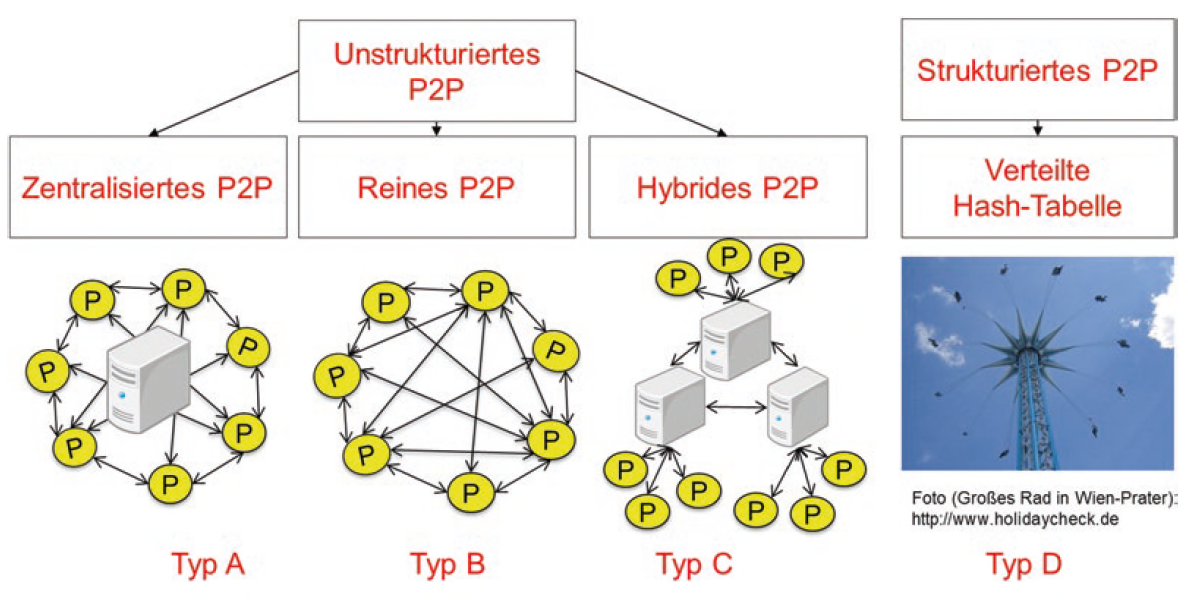
\includegraphics[width=1\linewidth]{images/peer_to_peer_typen.png}
    \captionof{figure}{Typen von Peer-to-Peer Netzwerken \parencite{Luntovskyy_ModRechnernetze}}
    \label{p2p_typen}
\end{center}

\noindent Unstrukturierte, strukturierte und hybride Peer-to-Peer Netzwerke sind unterschiedliche Ansätze zur Organisation von Knoten und Ressourcen in dezentralen Netzwerken. Unstrukturierte Netzwerke sind charakterisiert durch ihre fehlende explizite Organisationsstruktur, was eine einfache Konnektivität ermöglicht. Diese Netzwerke sind dynamisch und erlauben es Knoten frei beizutreten oder das Netzwerk zu verlassen, ohne die Gesamtstruktur signifikant zu beeinflussen. Die Suche nach Ressourcen oder Informationen erfolgt oft durch Broadcasts oder zufällige Weiterleitungen, was jedoch zu ineffizienten Suchprozessen führen kann, da keine klare Routing-Struktur vorhanden ist. Ein klassisches Beispiel für ein unstrukturiertes Netzwerk ist das Gnutella-Netzwerk, das sich durch seine dezentrale Natur auszeichnet, jedoch bei der effizienten Ressourcenlokalisierung Schwierigkeiten aufgrund des fehlenden organisierten Routings hat.

Strukturierte Peer-to-Peer Netzwerke hingegen weisen klare Regeln und Algorithmen zur Organisation der Knoten auf. Diese Netzwerke verfügen über eine explizite Organisationsstruktur, sei es eine Ringstruktur, k-bucket basierte Systeme oder andere, die es ermöglichen, effizientes Routing und eine optimierte Ressourcenverwaltung zu erreichen. Durch diese klar definierte Struktur sind strukturierte Netzwerke oft stabiler und bieten eine effizientere Ressourcenlokalisierung im Vergleich zu ihren unstrukturierten Gegenstücken. Allerdings kann diese Stabilität auf Kosten von Flexibilität und Anpassungsfähigkeit gehen, da Änderungen in der Netzwerktopologie oder hohe Dynamik der Knoten schwerer zu handhaben sind.

Hybride Peer-to-Peer Netzwerke versuchen, das Beste aus beiden Welten zu vereinen, indem sie Elemente aus strukturierten und unstrukturierten Ansätzen kombinieren. Diese Netzwerke integrieren Aspekte einer festen Organisationsstruktur für bestimmte Netzwerkbereiche, während andere Bereiche eher unstrukturiert sind. Als Beispiel hierfür kann Napster genannt werden, das eine oder mehrere Nodes dazu verwendet, um die Inhalte innerhalb des Netzwerks zu indizieren und zu verwalten, während der tatsächliche Download des Inhalts über eine direkte Verbindung zwischen den Teilnehmern erfolgt \parencite{Yang_ComparingHybridP2PSystems}.
Ziel ist es, Flexibilität und Effizienz zu optimieren und gleichzeitig eine gewisse Stabilität zu gewährleisten. Diese hybriden Ansätze streben danach, eine ausgewogene Lösung zu bieten, die sowohl die Anforderungen an eine stabile Struktur als auch an eine dynamische und flexible Umgebung erfüllt, je nach den spezifischen Bedürfnissen und Anwendungsfällen.

Um die Peer-to-Peer Funktionalität für das Protokoll dieser Arbeit zu gewährleisten, wird ein bereits existierendes Protokoll verwendet. In die engere Auswahl kamen Chord und Kademlia, welche beide lange Gegenstand intensiver Forschung waren, sowohl in der Industrie als auch in der akademischen Welt \parencite[S. 808]{MedranoChavez_ChordKademliaHighChurnScenarios}. 
Das Chord-Protokoll und das Kademlia-Protokoll sind zwei grundlegend verschiedene Ansätze zur Organisation von Peer-to-Peer Netzwerken. Beide Protokolle sind strukturiert und bieten eine effiziente Ressourcenlokalisierung, aber sie unterscheiden sich in ihrer Routing-Struktur und der Art und Weise, wie sie die Knoteninformationen verwalten.

Chord basiert auf einer Ringstruktur (siehe Abbildung \ref{chord_ring}), bei der die Knoten in einem Ring angeordnet sind und jeder Knoten für einen bestimmten Schlüsselbereich verantwortlich ist. Die Verbindungen zwischen den Knoten sind durch ihren Platz im Ring definiert, wobei jeder Knoten eine Verbindung zu seinem nächsten Nachbarn im Uhrzeigersinn hat. Bei der Suche nach einem bestimmten Schlüssel durchläuft eine Anfrage einen logarithmischen Pfad im Ring, wobei die Knoten auf dem Weg begrenzte Informationen über andere Knoten behalten, um Anfragen weiterzuleiten. Dieses Modell ist recht einfach und effizient für viele Anwendungsfälle, aber es könnte anfällig sein für Engpässe oder längere Suchzeiten, insbesondere wenn das Netzwerk dynamisch ist und sich die Konfiguration häufig ändert.

\begin{center}
    \captionsetup{type=figure}
    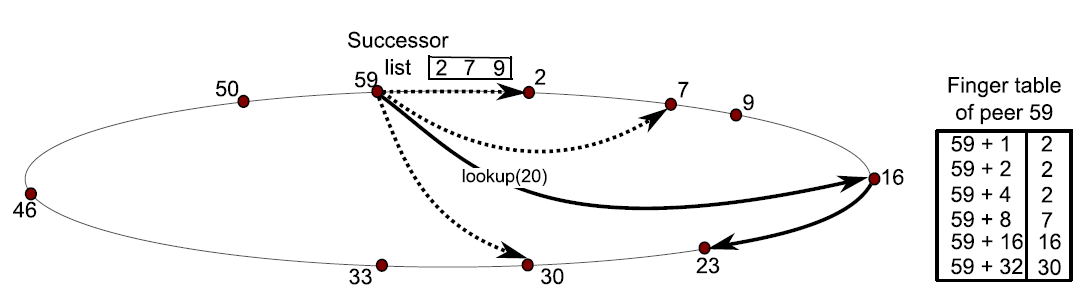
\includegraphics[width=0.9\linewidth]{images/chord_ring.png}
    \captionof{figure}{Visualisierung der Ringstruktur von Chord \parencite{MedranoChavez_ChordKademliaHighChurnScenarios}}
    \label{chord_ring}
\end{center}

\noindent Im Gegensatz dazu verwendet Kademlia eine K-Bucket-Struktur, die in Abbildung \ref{kademlia_tree} zu sehen ist, um eine effiziente Verwaltung von Knoteninformationen zu ermöglichen. Die K-Buckets enthalten eine Liste von Knoten für verschiedene Schlüsselbereiche basierend auf ihrer Nähe, die durch XOR-Distanzen der IDs berechnet wird. Die Verbindungen zwischen den Knoten sind asymmetrisch, und jeder Knoten speichert Informationen über andere Knoten in seinen K-Buckets. Bei der Suche nach einem bestimmten Schlüssel erfolgt das Routing durch die XOR-Entfernung, wodurch die nächsten Knoten für diesen Schlüssel gefunden werden. Dieses Verfahren ermöglicht ebenfalls eine logarithmische Anzahl von Schritten für die Suche und bietet eine robuste Struktur, die gut mit dynamischen Netzwerkänderungen umgehen kann.

\begin{center}
    \captionsetup{type=figure}
    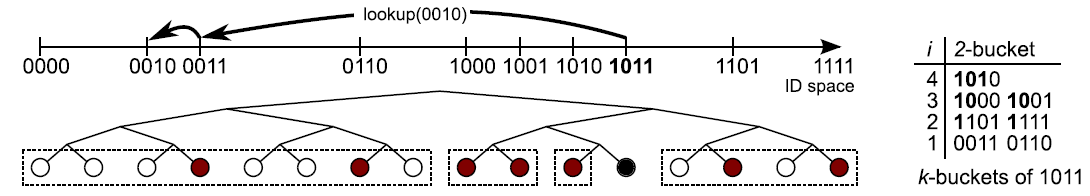
\includegraphics[width=0.9\linewidth]{images/kademlia_tree.png}
    \captionof{figure}{Visualisierung der Baumstruktur von Kademlia \parencite{MedranoChavez_ChordKademliaHighChurnScenarios}}
    \label{kademlia_tree}
\end{center}


\noindent Da bei einem Instant-Messaging Protokoll sehr häufig Teilnehmer das Netzwerk verlassen und neue Teilnehmer dem Netzwerk beitreten, ist es wichtig, dass das Protokoll mit hoher Fluktuation umgehen kann. Diese Fluktuation von Nodes wird als Churn (engl. Abwanderung) bezeichnet. In einer Studie von Medrano-Chávez et al. \parencite{MedranoChavez_ChordKademliaHighChurnScenarios}, welche im hybriden Journal \textit{Peer-to-Peer Networking and Applications} veröffentlicht wurde, wurde die Leistung von Chord und Kademlia in Bezug auf Netzwerkfluktuation untersucht. Die Ergebnisse zeigen, dass Kademlia bei hoher Fluktuation besser abschneidet als Chord. Aus diesem Grund wird Kademlia als Grundlage für das Protokoll verwendet.

Um die Problematik mit Firewalls und NAT-Gateways zu lösen, wird ein TCP-Relay verwendet. Dieses ist ein Server, der die Nachrichten weiterleitet, wenn der Empfänger nicht direkt erreichbar ist. Der Server ist nur für die Weiterleitung der Nachricht zuständig und speichert diese nicht. Das hier entworfene Protokoll bietet keine Möglichkeit, Nachrichten zu speichern, wenn der Empfänger offline ist. Bei der Verwendung dieses Protokolls in einer realen Anwendung könnte eine Funktion implementiert werden, die es wiederholt versucht, die Nachricht zu senden, bis der Empfänger wieder online ist. Die genauere Implementierung dieser Funktion ist jedoch nicht Teil dieser Arbeit und ist dem Entwickler überlassen.




\subsection{Identifikation von Teilnehmern}
\label{subsec:identifikation_von_teilnehmern}


\begin{itemize}
    \item Jeder Benutzer im Netzwerk hat eine eindeutige ID.
    \item Adressierung kann über Benutzer-IDs oder Schlüsselpaare erfolgen.
    \item Die ID wird als 32-Byte-Array gespeichert.
\end{itemize}

[Jeder Benutzer im Netzwerk hat eine eindeutige ID. Adressierung kann über 
Benutzer-IDs oder Schlüsselpaare erfolgen.]

\noindent Da es in Peer-to-Peer-Netzwerken keinen zentralen Server gibt, der die
Kommunikation steuert, müssen die Teilnehmer auf andere Weise identifiziert
werden. Hierfür können verschiedene Methoden zur
Identifizierung von Teilnehmern verwendet werden. Für dieses Protokoll
fiel die Wahl auf das Kademlia-Protokoll, das in vielen Peer-to-Peer-Netzwerken
verwendet wird. Das Kademlia-Protokoll verwendet eine ID mit einer Länge von 160
Bit, die durch einen \textcolor{red}{SHA-1-Hash} des öffentlichen Schlüssels des 
Teilnehmers erzeugt wird. Durch die Verwendung einer Hashfunktion wird die ID auf eine
festgelegte Länge begrenzt.


\subsection{Nachrichtenformat}

Struktur für Nachrichten festlegen (Header, Body, etc.).
Verschlüsselung und Authentifizierung für Sicherheit hinzufügen.
Jedes Instant Messaging-Protokoll benötigt die Definition eines Nachrichtenformats,
das die Struktur der Nachrichten festlegt, die zwischen den Teilnehmern ausgetauscht werden.
Dieses Nachrichtenformat sollte die folgenden Elemente enthalten:

\noindent Nachrichtenkopf:
\begin{itemize}
    \item Absender-ID: Eindeutige Kennung des Absenders (Benutzername? Public Key?)
    \item Empfänger-ID: Identifikation des Empfängers (Benutzername? Public Key?)
    \item Zeitstempel: Zeitpunkt, zu dem die Nachricht gesendet wurde
    \item Nachrichten-ID: Eindeutige Kennung der Nachricht für die Identifikation 
    und Verfolgung
\end{itemize}

Im Nachrichtenkopf müssen sich die Absender- und Empfänger-IDs befinden,
um die Kommunikation zwischen den Teilnehmern zu ermöglichen.
Die Nachrichten-ID ist erforderlich, um die Nachrichten zu identifizieren und
die Zustellung zu verfolgen. Der Zeitstempel ist hilfreich, um die Nachrichten
zu sortieren und die Reihenfolge der Nachrichten zu bestimmen.


\noindent Nachrichteninhalt:
\begin{itemize}
    \item Textinhalt: Der eigentliche Text der Nachricht
    \item Formatierung: Möglicherweise könnte man einfache Formatierungsoptionen 
    unterstützen, z. B. fett, kursiv, Unterstreichungen usw.
\end{itemize}

Der Nachrichteninhalt sollte den eigentlichen Text der Nachricht enthalten.


\noindent Zusätzliche Tags:
\begin{itemize}
    \item Priorität: Wenn Nachrichten eine Priorität haben sollen, könnte 
    man Tags oder Flags einführen, um die Wichtigkeit zu markieren 
    (z. B. "Dringend", "Normal", "Niedrige Priorität")
\end{itemize}


\noindent Zustellbestätigung:
\begin{itemize}
    \item Eine Option für eine Bestätigung der Nachrichtenzustellung könnte 
    hilfreich sein, um sicherzustellen, dass die Nachricht erfolgreich 
    übermittelt wurde
\end{itemize}


\noindent Unicode-Unterstützung:
\begin{itemize}
    \item Unterstützung erforderlich, um eine breite Palette von Sprachen und
    Zeichen darstellen zu können
\end{itemize}

\noindent Verschlüsselung und Sicherheit:
\begin{itemize}
    \item Verschlüsselung und Authentifizierung erforderlich, um 
    die Vertraulichkeit der Nachrichten zu gewährleisten
\end{itemize}

\subsection{Routing und Peer Discovery}
\label{subsec:routing}

Wie bereits in Abschnitt \ref{subsec:identifikation_von_teilnehmern} 
\nameref{subsec:identifikation_von_teilnehmern} erwähnt,
wird das Kademlia-Protokoll verwendet, um die Knoten im Netzwerk zu identifizieren.
Es wird auch verwendet, um die Nachrichten zwischen den Knoten zu routen.

% Wenn ein Knoten einen Wert oder einen anderen Knoten im Netzwerk finden möchte, 
% führt er iterative Suchen durch, indem er eine auf XOR basierende Distanzmetrik 
% verwendet. Er fragt Knoten in seiner Routing-Tabelle basierend auf ihrer Nähe 
% zur Zielknoten-ID ab. Diese Abfragen helfen, die Suche auf das Ziel hin zu verfeinern, 
% indem sie sich mit jedem Schritt im Knoten-ID-Raum näher bewegen. Die iterative
% Suche wird beendet, wenn der Zielknoten gefunden wurde oder wenn die Suche
% keine Knoten mehr findet, die der Zielknoten-ID näher sind als der am nächsten
% gelegene Knoten, der bereits abgefragt wurde. In diesem Fall wird die Suche
% beendet und der am nächsten gelegene Knoten zurückgegeben.

% Im Kademlia-Protokoll sind vier Funktionen definiert, die für die Suche nach
% Knoten und Werten verwendet werden. Diese Funktionen sind \texttt{FIND\_NODE},
% \texttt{FIND\_VALUE}, \texttt{PING} und \texttt{STORE}. Die Funktionen
% \texttt{FIND\_NODE} und \texttt{FIND\_VALUE} werden verwendet, um nach Knoten
% oder Werten zu suchen. Die Funktion \texttt{PING} wird verwendet, um die
% Erreichbarkeit eines Knotens zu überprüfen. Die Funktion \texttt{STORE} wird
% verwendet, um einen Wert in einem Knoten zu speichern.


Das Kademlia-Protokoll basiert auf einem Distanzmetrik-Konzept, das als \\
"Kademlia-Distanz" bekannt ist. Jeder Knoten im Netzwerk wird durch eine eindeutige ID repräsentiert, 
typischerweise als kryptografischer Hashwert, der sich aus der gehashten IP-Adresse 
des jeweiligen Knotens mittels der SHA-1 Hashfunktion ergibt. Diese IDs sind in einem 
großen binären Baum organisiert, wobei die Position eines Knotens im Baum seine 
"Kademlia-Distanz" zu anderen Knoten definiert. Diese Distanz wird durch die XOR 
(ausschließendes Oder)-Operation ihrer eindeutigen IDs bestimmt. Die XOR-Operation 
ermöglicht eine effiziente Bestimmung der Distanz zwischen den Knoten-IDs, indem 
sie auf deren Binärzahlen angewendet wird. Dieses Ergebnis repräsentiert die 
Distanz zwischen den IDs und bildet die Grundlage für das Routing und die 
Organisation im Kademlia-Netzwerk.

Kademlia verwendet ein Routingverfahren, bei dem jeder Knoten eine Routing-\\
Tabelle 
speichert, die als "K-Buckets" bezeichnet werden. Jedes K-Bucket enthält Verweise 
auf andere Knoten im Netzwerk und ist nach der Kademlia-Distanz organisiert. Ein 
K-Bucket enthält typischerweise eine begrenzte Anzahl von Einträgen und gruppiert 
Knoten mit ähnlichen IDs.

Wenn ein Knoten eine Verbindung zu einem anderen Knoten herstellen muss, verwendet 
er die Routing-Tabelle, um den am nächsten gelegenen Knoten zu finden, der die 
Ziel-ID repräsentiert. Falls dieser Knoten nicht direkt bekannt ist, wird das 
Routing iterative durchgeführt, wobei der Knoten jeweils näher an der Ziel-ID 
liegende Knoten anfragt, bis der Zielknoten gefunden wird. Durch die Verwendung 
dieses strukturierten Ansatzes ermöglicht Kademlia eine effiziente Suche und 
Kommunikation zwischen Knoten in einem P2P-Netzwerk, wobei die Skalierbarkeit 
und Robustheit des Systems erhalten bleiben. Es ist ein Schlüsselelement vieler 
P2P-Anwendungen, einschließlich Filesharing, dezentraler Datenbanken und eben auch 
Instant Messaging-Protokollen, da es die Grundlage für die direkte 
Peer-to-Peer-Kommunikation schafft.
\\

\noindent Ein Beispiel für die XOR-Berechnung zwischen gehashten Knoten-IDs könnte wie folgt 
aussehen:
Knoten A hat die gehashte ID: 0x83a2c8f7,  
Knoten B hat die gehashte ID: 0xe1b6d4a9.

\noindent Die XOR-Operation zwischen diesen IDs ergibt:
\begin{equation}
    \begin{aligned}
        \text{Knoten A:} & \quad \texttt{0x83a2c8f7} \\
        \text{Knoten B:} & \quad \texttt{0xe1b6d4a9} \\
        \text{Ergebnis:} & \quad \texttt{0x61f47c5e}
    \end{aligned}
\end{equation}
% #TODO: Berechnung noch in binär umwandeln, damit die Berechnung besser verständlich ist?


\noindent Diese Distanz repräsentiert die Maßeinheit für die Positionierung und das Routing 
im Kademlia-Netzwerk. Knoten mit einer geringeren Distanz sind näher beieinander
als Knoten mit einer größeren Distanz. Dabei hat die Distanz nichts mit der
geographischen Entfernung zu tun, sondern nur mit der Position im Kademlia-Baum.

\subsection{Status- und Präsenzinformationen}

Definieren Sie, wie Benutzer ihren Status aktualisieren (Online, Abwesend, Offline).
Überlegungen zur Präsenzinformation für effiziente Nachrichtenzustellung.

\subsection{Verbindungsmanagement}

Mechanismen für den Aufbau und die Beendigung von Peer-Verbindungen. Pufferung von Nachrichten für offline Benutzer.

Die Herstellung einer Verbindung zwischen zwei Teilnehmern ist ein wichtiger Aspekt eines Instant Messaging-Protokolls. Der Benutzer, der eine Verbindung aufbauen möchte, muss die eindeutige ID des anderen Benutzers kennen. DieseID wird verwendet, um eine Suche im Kademlia-Netzwerk durchzuführen, um den Knoten zu finden, der den Benutzer repräsentiert. Wenn der Knoten gefunden wurde, kann eine Verbindung hergestellt werden, indem eine Verbindungsanfrage gesendet wird. Wenn der Knoten die Anfrage akzeptiert, wird eine direkte Verbindung zwischen den beiden Knoten hergestellt. Wenn die Verbindung erfolgreich hergestellt wurde, können die Teilnehmer Nachrichten austauschen. Sollte der gesuchte Knoten nicht gefunden werden, wird auf ein TCP-Relay zurückgegriffen, um die Nachricht zu übermitteln. Dieses Relay ist ein Server, der die Nachrichten zwischen den Teilnehmern weiterleitet. Dieser Mechanismus wird verwendet, wenn die direkte Verbindung zwischen den Teilnehmern nicht möglich ist, z. B. wenn sich die Teilnehmer hinter einer Firewall befinden. Die Verwendung eines TCP-Relays ist jedoch nicht wünschenswert, da es die Skalierbarkeit des Systems beeinträchtigt und die Vertraulichkeit der Nachrichten gefährdet. Daher sollte die direkte Verbindung zwischen den Teilnehmern bevorzugt werden.


%\subsection{Verbindung und Identität}

Benutzer können andere Peers in einem verteilten Netzwerk entdecken und sich mit ihnen 
verbinden. Dies kann verteilte Hash-Tabellen (DHTs) oder andere Mechanismen zur 
Peer-Erkennung umfassen.
Benutzer werden durch eindeutige öffentliche Schlüssel identifiziert, und Benutzerprofile 
können zusätzliche Informationen wie Benutzernamen, Avatare und Status enthalten.

%\subsection{Nachrichten und Daten}

Benutzer können ausschließlich Textnachrichten miteinander austauschen. 
Diese Nachrichten können an einzelne Peers gesendet werden.
Die gesamte Kommunikation ist mit starken Verschlüsselungsalgorithmen 
verschlüsselt, um Privatsphäre und Sicherheit zu gewährleisten.

%\subsection{Nachrichtenverlauf}

Benutzer haben die Möglichkeit, ihren Nachrichtenverlauf lokal zu speichern.
Der Nachrichtenverlauf ist ebenfalls verschlüsselt, um die Sicherheit zu gewährleisten.

\subsection{Sicherheit}

Alle Nachrichten sind mit öffentlichen Schlüsseln verschlüsselt, um sicherzustellen, 
dass nur der beabsichtigte Empfänger die Nachrichten entschlüsseln und lesen kann.
Ein sicheres Verfahren für den Schlüsselaustausch und die Schlüsselverwaltung 
wird implementiert, um gegen Abhören und Man-in-the-Middle-Angriffe zu schützen.

\subsection{Fehlerbehandlung}

Fehlerbehandlung und -vermeidung sind wichtige Aspekte eines Instant Messaging-Protokolls. Fehler können zu einer Unterbrechung der Verbindung zwischen den Teilnehmern führen. Um dies zu verhindern, werden verschiedene Mechanismen implementiert, die die Verbindung zwischen den Teilnehmern aufrechterhalten.

Netzwerkfehler können zu einer Unterbrechung der Verbindung zwischen den Teilnehmern führen. Um dies zu verhindern, wird eine Pufferung der Nachrichten implementiert. Wenn ein Teilnehmer eine Nachricht sendet, wird diese in einem Puffer gespeichert, bis der Empfänger die Nachricht empfangen hat. Wenn der Empfänger die Nachricht nicht empfangen kann, wird sie im Puffer gespeichert, bis der Empfänger wieder online ist. Wenn der Empfänger wieder online ist, wird die Nachricht erneut gesendet. Wenn der Empfänger die Nachricht empfangen hat, wird sie aus dem Puffer gelöscht. Wenn der Empfänger die Nachricht nicht empfangen kann, wird sie nach einer bestimmten Zeit aus dem Puffer gelöscht. Die Pufferung der Nachrichten ermöglicht es, die Verbindung zwischen den Teilnehmern aufrechtzuerhalten, auch wenn einer der Teilnehmer offline ist. Dies ist ein wichtiger Aspekt für ein Instant Messaging-Protokoll, da die Teilnehmer nicht immer online sind. 
\\
\\
Firewall und NAT können ebenfalls zu Verbindungsproblemen führen. Um dies zu verhindern, wird ein TCP-Relay verwendet, um die Nachrichten zwischen den Teilnehmern weiterzuleiten. Dieser Mechanismus wird verwendet, wenn die direkte Verbindung zwischen den Teilnehmern nicht möglich ist, z. B. wenn sich die Teilnehmer hinter einer Firewall befinden. Die Verwendung eines TCP-Relays ist jedoch nicht wünschenswert, da es die Skalierbarkeit des Systems beeinträchtigt und die Vertraulichkeit der Nachrichten gefährdet. Daher sollte die direkte Verbindung zwischen den Teilnehmern bevorzugt werden.
\\
\\
Peer-spezifische Fehler:
\\
\\
In einem Peer to Peer Netzwerk kann es häufig vorkommen, dass der gewünschte Teilnehmer nicht online und somit nicht Teil des Netzwerks ist. In diesem Fall wird eine Fehlermeldung an den Absender zurückgegeben, dass der gewünschte Teilnehmer nicht gefunden werden konnte. Wie diese Fehlermeldung implementiert wird, ist dem Entwickler überlassen. Ein weiterer Fehler könnte im Zusammenhang mit Authentifizierung entstehen. Wenn ein Teilnehmer eine Nachricht an einen anderen Teilnehmer senden möchte, muss er sich zuerst authentifizieren. Die Authentifizierung erfolgt über die Blockchain, indem der öffentliche Schlüssel des Teilnehmers mit der ID des Teilnehmers verglichen wird. Wenn die IDs übereinstimmen, ist der Teilnehmer authentifiziert und die Nachricht kann gesendet werden. Wenn die IDs nicht übereinstimmen, ist der Teilnehmer nicht authentifiziert und die Nachricht wird nicht gesendet. In diesem Fall wird eine Fehlermeldung an den Absender zurückgegeben, dass der Teilnehmer nicht authentifiziert ist. Wie diese Fehlermeldung implementiert wird, ist dem Entwickler überlassen.
\\
\\
Nachrichtenbezogene Fehler:
\\
\\
Es besteht die Möglichkeit, dass Teile von Nachrichten oder auch ganze Nachrichten verloren gehen können. Da Kademlia über UDP läuft, hat es nicht die Möglichkeiten, die beispielsweise TCP bietet. TCP kann bei Paketverlust die Pakete erneut senden, UDP kann dies nicht. Zusätzlich können Nachrichten beschädigt werden (\textcolor{red}{Prüfsumme?}).
